\documentclass{beamer}

\usepackage[utf8]{inputenc}
\usepackage{hyperref}
%\usepackage{lmodern}

\usepackage{listings}
\definecolor{mygreen}{RGB}{28,172,0} % color values Red, Green, Blue
\lstdefinestyle{limpo}{numbers=none}
\lstset{language=TeX,
    basicstyle=\small,
    commentstyle=\color{mygreen},%
    numbers=left,%
    numberstyle={\small \color{black}},% size of the numbers
    numbersep=9pt, % this defines how far the numbers are from the text
    emph=[1]{documentclass,usepackage,begin,end},emphstyle=[1]\color{blue}, %some words to emphasise
}

\newcommand{\tbs}{\textbackslash}

\author[Adriano Barbosa]{Prof. Adriano Oliveira Barbosa}
\title{Introdu\c{c}\~ao ao \LaTeX}
\subtitle[Semana da Matem\'atica]{VII Semana Acad\^emica da Matem\'atica UFGD}
\date{Agosto, 2018}

\beamertemplatenavigationsymbolsempty
%\usetheme{Warsaw}
%\setbeamercolor{normal text}{fg=white,bg=black!90}
%\setbeamercolor{structure}{fg=white}
%\setbeamercolor{alerted text}{fg=red!85!black}
%\setbeamercolor{item projected}{use=item,fg=black,bg=item.fg!35}
%\setbeamercolor*{palette primary}{use=structure,fg=structure.fg}
%\setbeamercolor*{palette secondary}{use=structure,fg=structure.fg!95!black}
%\setbeamercolor*{palette tertiary}{use=structure,fg=structure.fg!90!black}
%\setbeamercolor*{palette quaternary}{use=structure,fg=structure.fg!95!black,bg=black!80}
%\setbeamercolor*{framesubtitle}{fg=white}
%\setbeamercolor*{block title}{parent=structure,bg=black!60}
%\setbeamercolor*{block body}{fg=black,bg=black!10}
%\setbeamercolor*{block title alerted}{parent=alerted text,bg=black!15}
%\setbeamercolor*{block title example}{parent=example text,bg=black!15}

\begin{document}

\begin{frame}
	\maketitle
\end{frame}

\begin{frame}{O que \'e o \LaTeX?}
    O \TeX \'e um sistema de tipografia criado por Donald Knuth em 1978.

    \vspace{1cm}
    \pause

    \LaTeX \'e um conjunto de macros para o \TeX, utilizado amplamente na
    produ\c{c}\~ao de textos matem\'aticos e cient\'{\i}ficos, devido a sua alta qualidade
    tipogr\'afica.
\end{frame}

\begin{frame}[fragile]{Software necess\'ario}
    Um \textbf{editor}\footnote{O MS Word \'e um \textbf{processador} de texto.} de
    texto ou um editor especializado para (La)TeX
        \begin{enumerate}
            \item Texmaker (\url{http://www.xm1math.net/texmaker/}) \\ GNU/Linux, BSDs, Windows e Mac OS
            \item Kile (\url{https://kile.sourceforge.io/})\\ GNU/Linux e BSDs
            \item TeXnicCenter (\url{http://www.texniccenter.org/})\\ MS Windows
            \item TeXShop (\url{http://pages.uoregon.edu/koch/texshop/})\\ Mac OS
        \end{enumerate}

    \vspace{1cm}
    Uma lista mais completa de editores est\'a dispon\'{\i}vel em:
    \url{http://www.tug.org/interest.html#packages}
\end{frame}

\begin{frame}[fragile]{Software necess\'ario}
    Uma distribui\c{c}\~ao (La)TeX
        \begin{enumerate}
            \item TeX Live (\url{https://tug.org/texlive/})\\ GNU/Linux, BSDs e MS Windows
            \item MacTeX (\url{http://www.tug.org/mactex/})\\ Mac OS
            \item MiKTeX (\url{https://miktex.org/})\\ MS Windows
        \end{enumerate}

    \vspace{1cm}
    Uma lista mais completa de distrubui\c{c}\~oes est\'a dispon\'{\i}vel em:
    \url{http://www.tug.org/interest.html#free}
\end{frame}

\begin{frame}{Instala\c{c}\~ao do Texmaker (MS Windows)}
    \begin{figure}[h]
        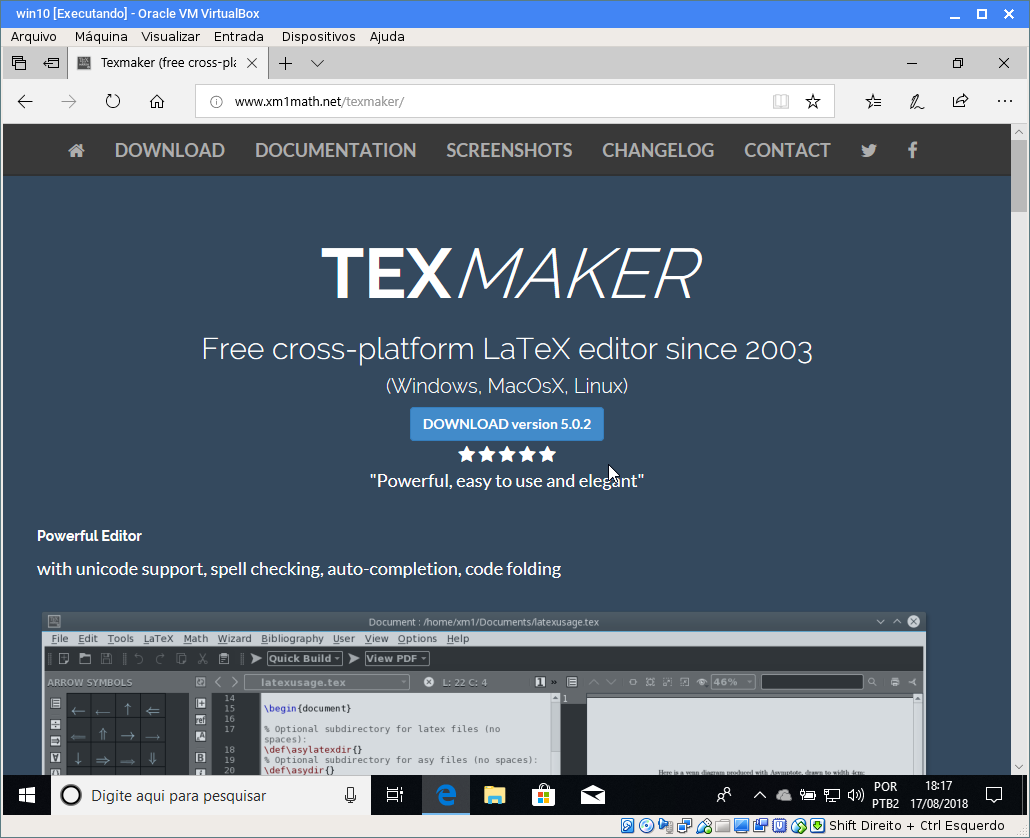
\includegraphics[scale=0.25]{fig/texmaker-site.png}
    \end{figure}
\end{frame}

\begin{frame}{Instala\c{c}\~ao do Texmaker (MS Windows)}
    \begin{figure}[h]
        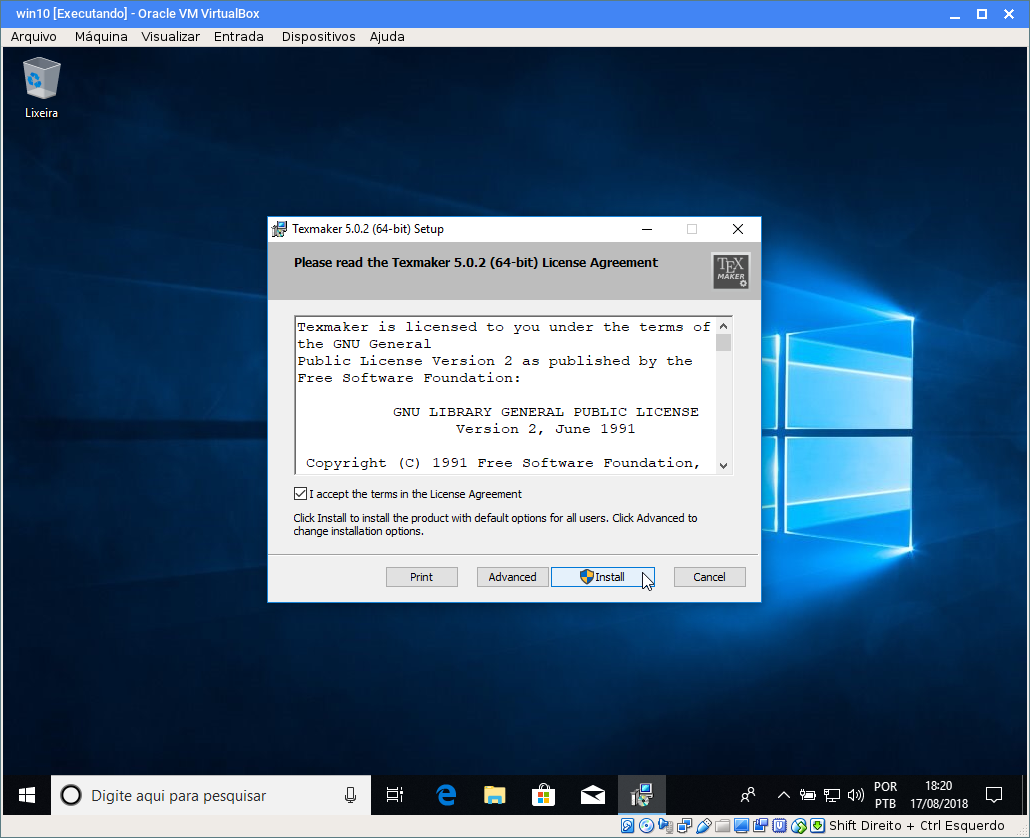
\includegraphics[scale=0.25]{fig/texmaker-01.png}
    \end{figure}
\end{frame}

\begin{frame}{Instala\c{c}\~ao do Texmaker (MS Windows)}
    \begin{figure}[h]
        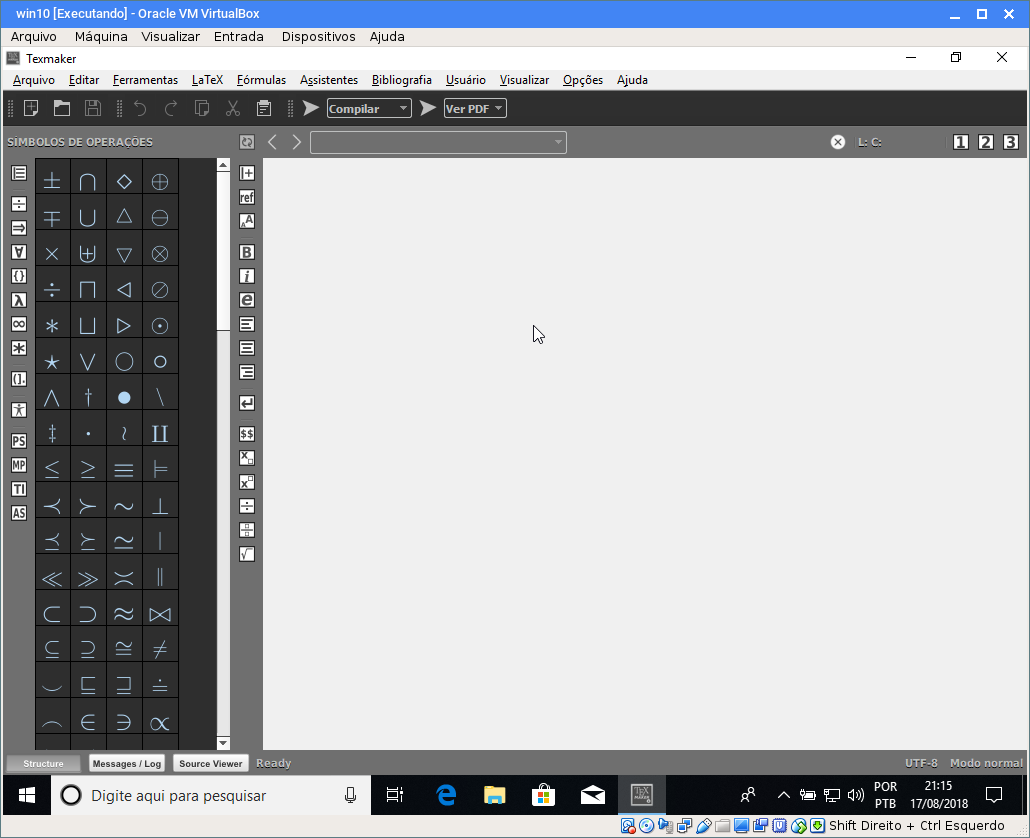
\includegraphics[scale=0.25]{fig/texmaker-02.png}
    \end{figure}
\end{frame}

\begin{frame}{Instala\c{c}\~ao da distribui\c{c}\~ao (MS Windows)}
    \begin{figure}[h]
        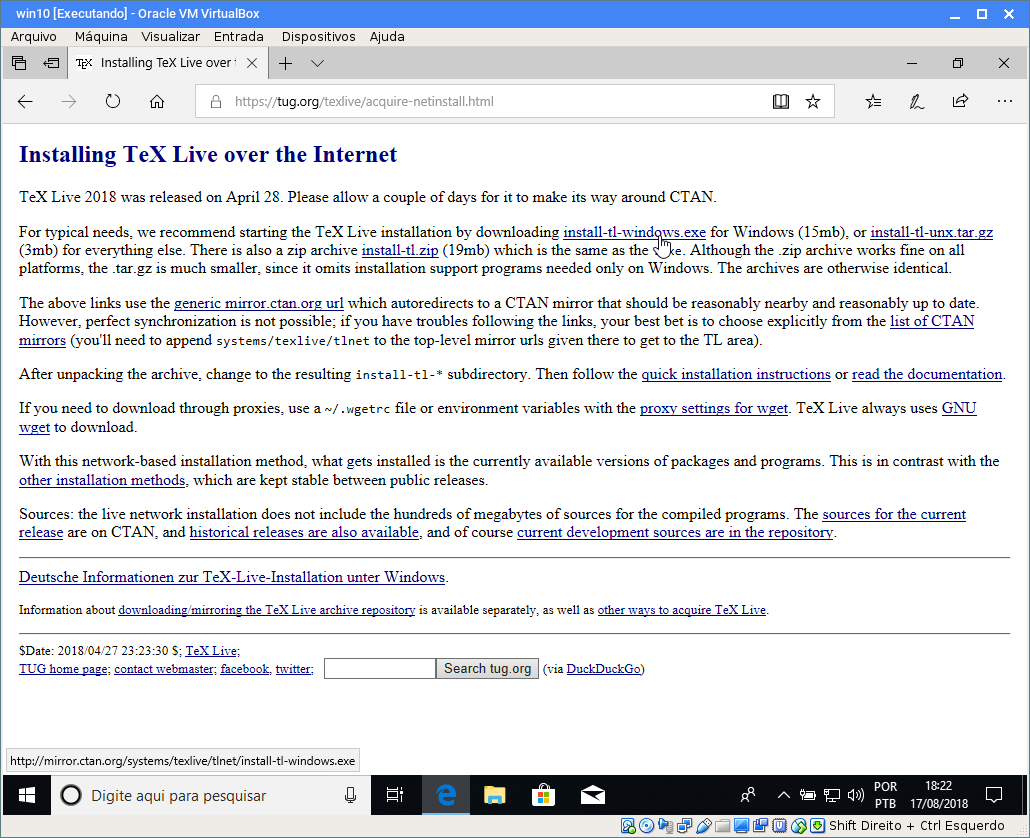
\includegraphics[scale=0.25]{fig/texlive-site.png}
    \end{figure}
\end{frame}

\begin{frame}{Instala\c{c}\~ao da distribui\c{c}\~ao (MS Windows)}
    \begin{figure}[h]
        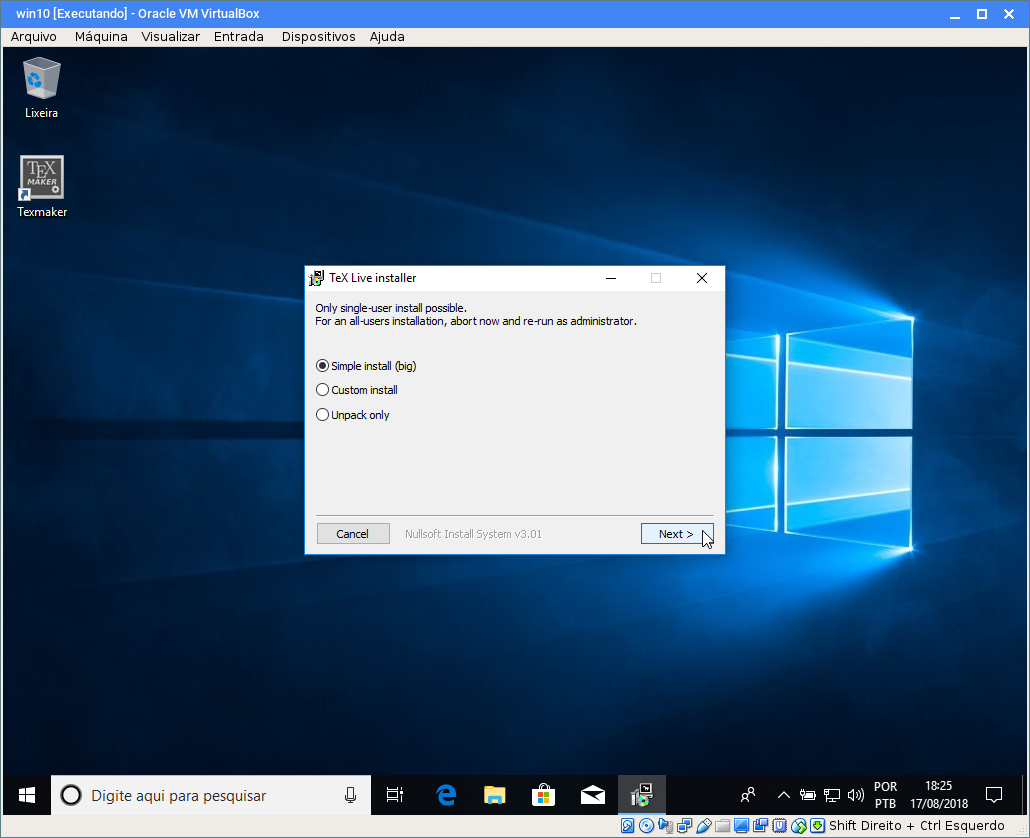
\includegraphics[scale=0.25]{fig/texlive-01.png}
    \end{figure}
\end{frame}

\begin{frame}{Instala\c{c}\~ao da distribui\c{c}\~ao (MS Windows)}
    \begin{figure}[h]
        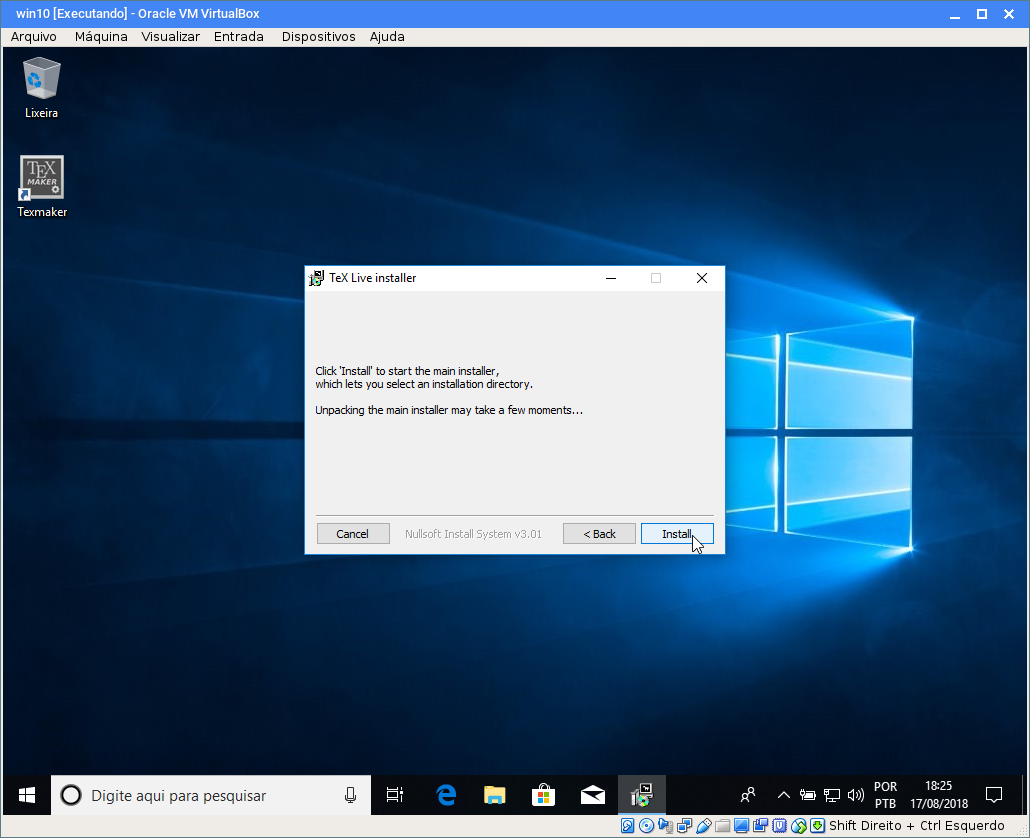
\includegraphics[scale=0.25]{fig/texlive-02.png}
    \end{figure}
\end{frame}

% \begin{frame}{Instala\c{c}\~ao da distribui\c{c}\~ao (MS Windows)}
%     \begin{figure}[h]
%         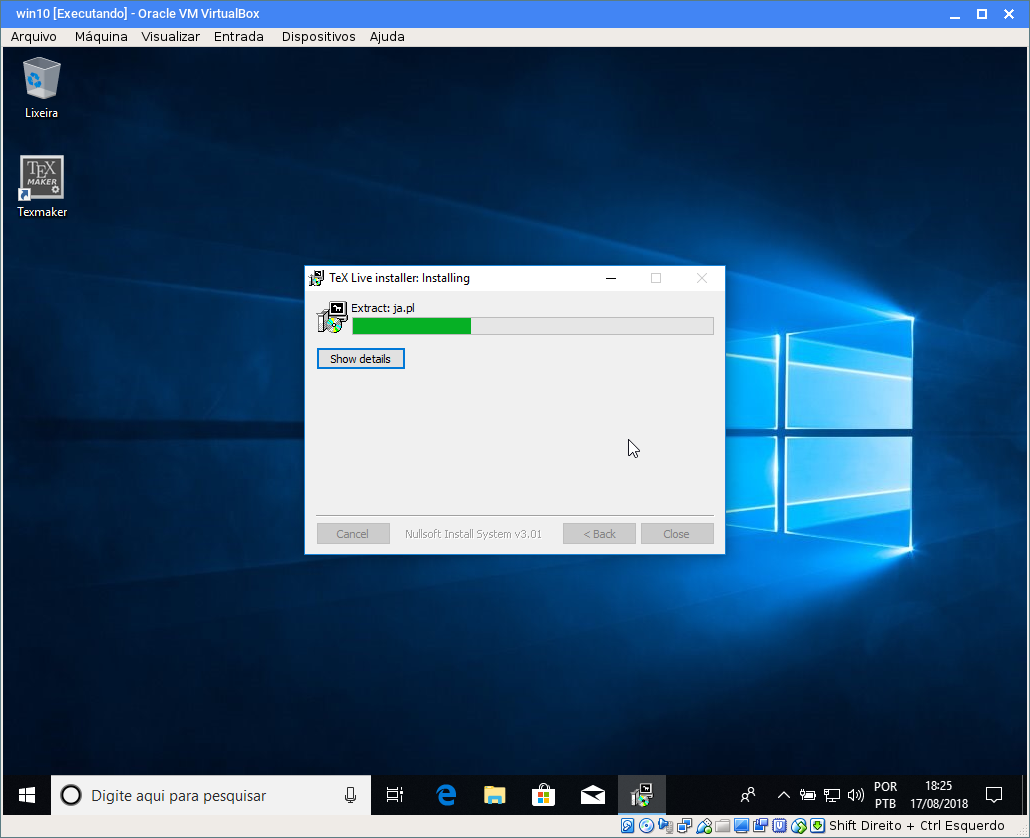
\includegraphics[scale=0.25]{fig/texlive-03.png}
%     \end{figure}
% \end{frame}

\begin{frame}{Instala\c{c}\~ao da distribui\c{c}\~ao (MS Windows)}
    \begin{figure}[h]
        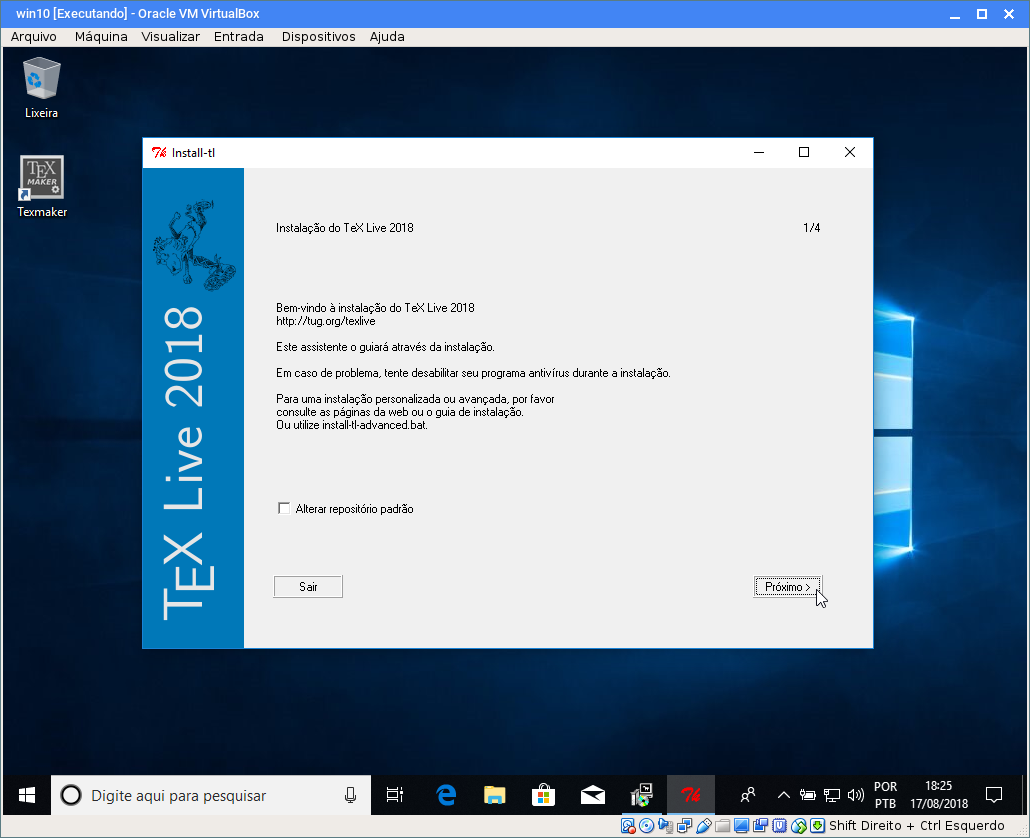
\includegraphics[scale=0.25]{fig/texlive-04.png}
    \end{figure}
\end{frame}

\begin{frame}{Instala\c{c}\~ao da distribui\c{c}\~ao (MS Windows)}
    \begin{figure}[h]
        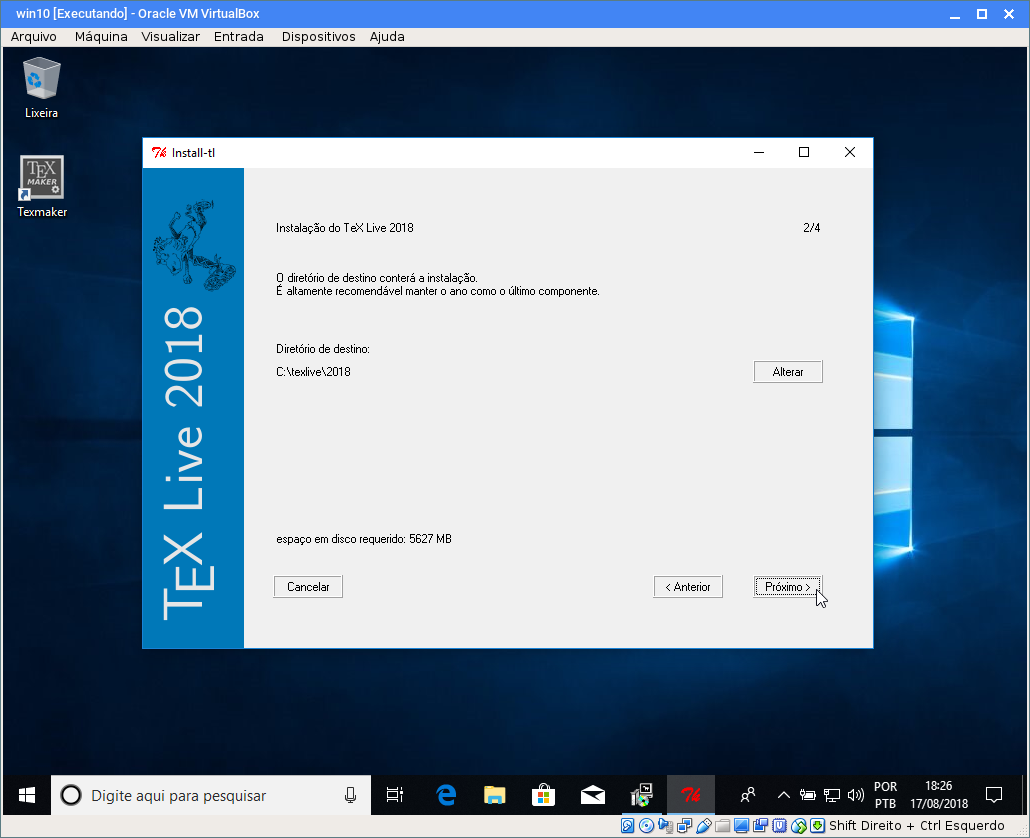
\includegraphics[scale=0.25]{fig/texlive-05.png}
    \end{figure}
\end{frame}

\begin{frame}{Instala\c{c}\~ao da distribui\c{c}\~ao (MS Windows)}
    \begin{figure}[h]
        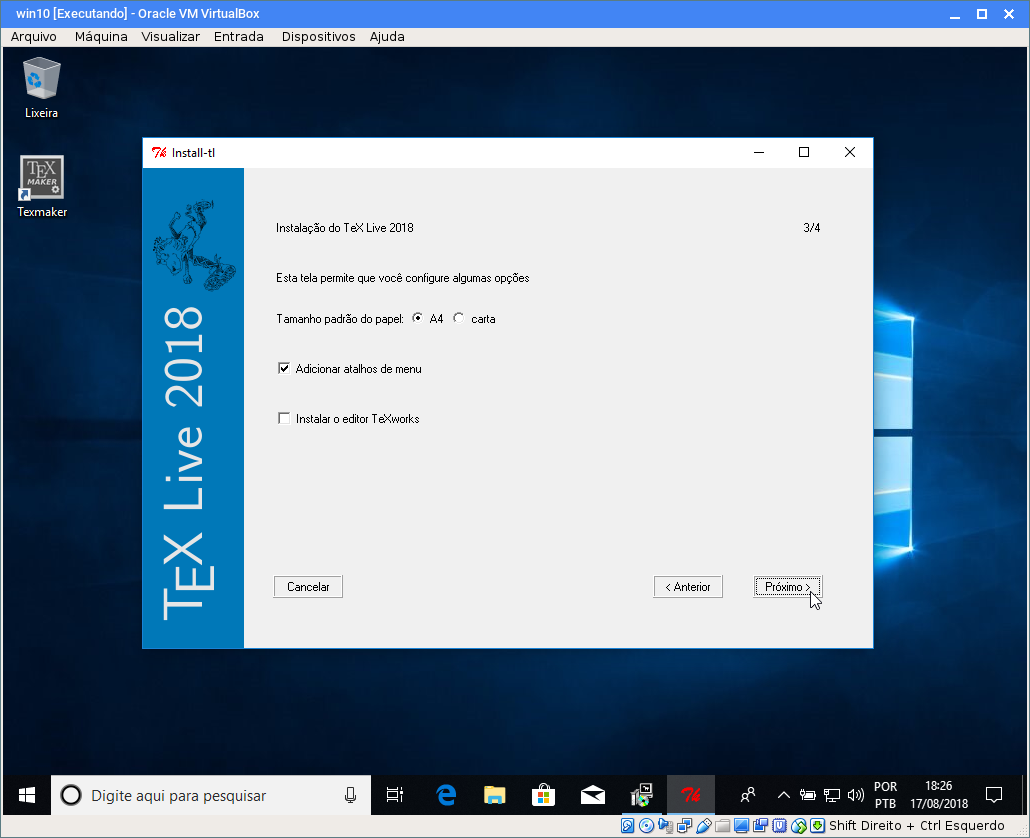
\includegraphics[scale=0.25]{fig/texlive-06.png}
    \end{figure}
\end{frame}

\begin{frame}{Instala\c{c}\~ao da distribui\c{c}\~ao (MS Windows)}
    \begin{figure}[h]
        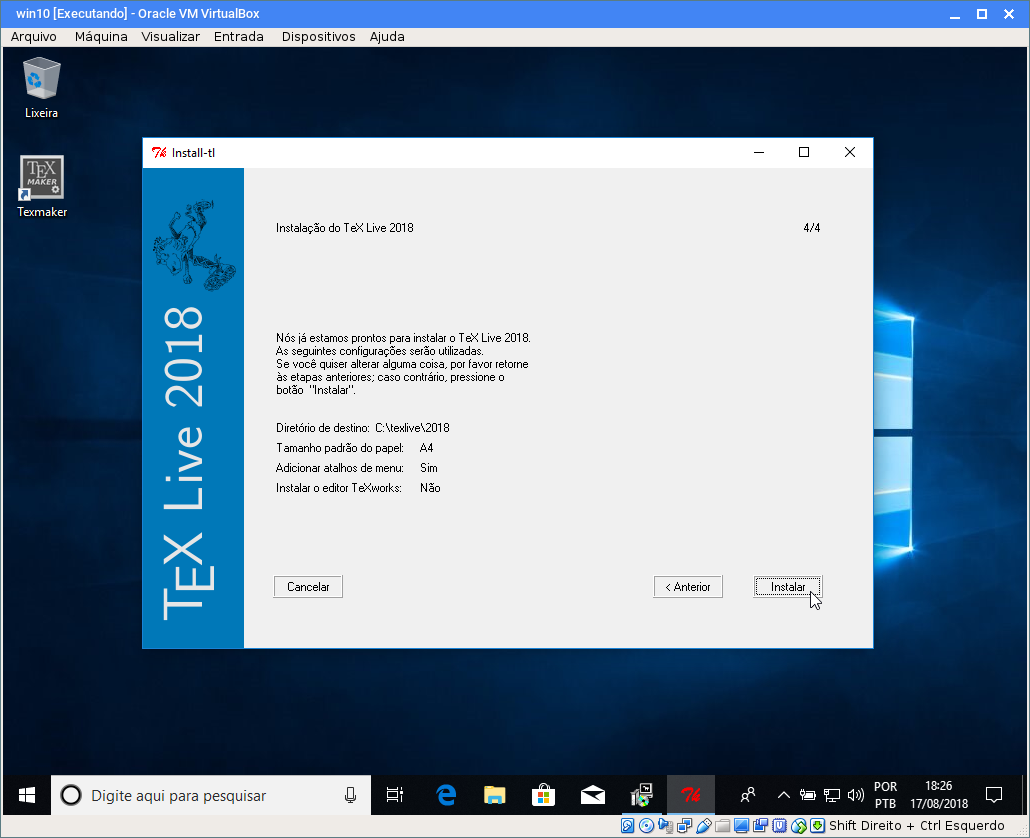
\includegraphics[scale=0.25]{fig/texlive-07.png}
    \end{figure}
\end{frame}

\begin{frame}{Instala\c{c}\~ao da distribui\c{c}\~ao (MS Windows)}
    \begin{figure}[h]
        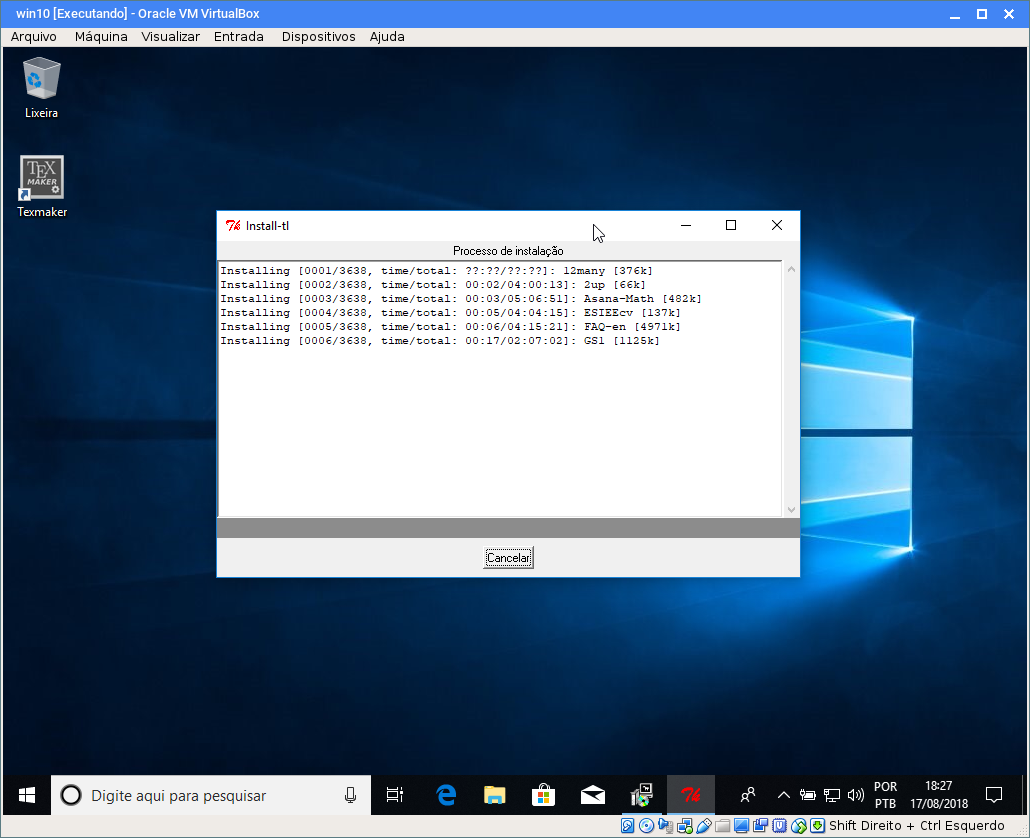
\includegraphics[scale=0.25]{fig/texlive-08.png}
    \end{figure}
\end{frame}

\begin{frame}{Instala\c{c}\~ao do Texmaker e da distrubiu\c{c}\~ao (GNU/Linux)}
    Debian/Ubuntu: sudo apt-get install texmaker texlive-full
    Fedora/Redhat: sudo yum install texmaker texlive-scheme-full
\end{frame}

\begin{frame}{O processo}
    \begin{figure}[h]
        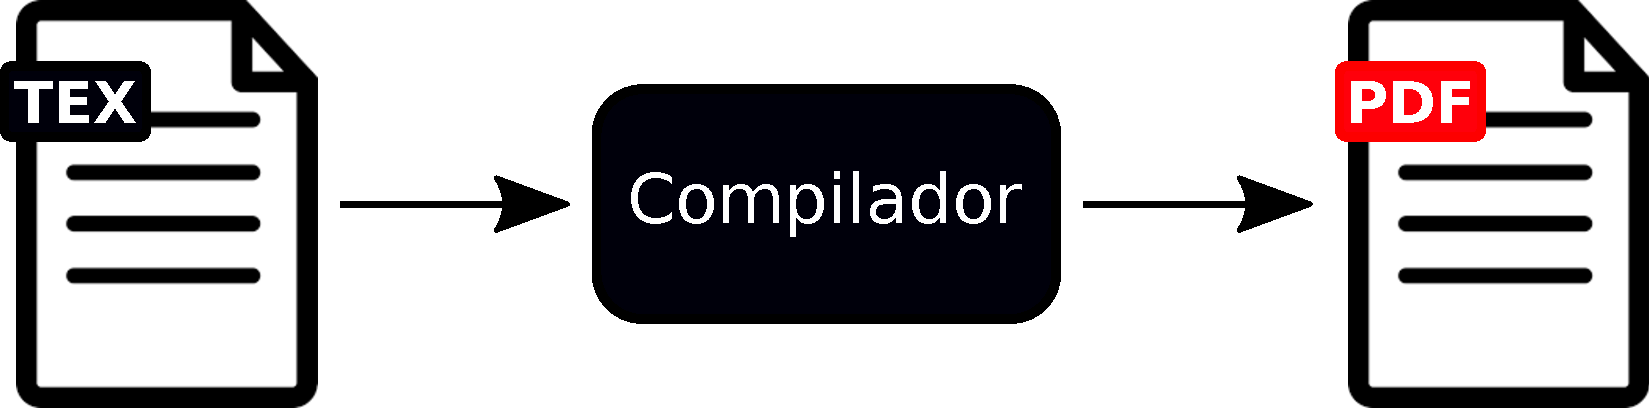
\includegraphics[width=\textwidth]{fig/pipeline.pdf}
    \end{figure}
\end{frame}

\begin{frame}{Vocabul\'ario}
    \begin{itemize}
        \item .tex: arquivo (La)TeX (aquele que vamos escrever)
        \item .dvi: acr\^onimo para DeVice-Independent
        %\item .ps: linguagem PostScript %(linguagem de descri\c{c}\~ao de p\'aginas, originalmente criada para impress\~ao e posteriormente modificada para o uso com monitores)
        \item .pdf: Portable Document Format
        \item compilador\footnote{O processo de compila\c{c}\~ao tamb\'em gera outros
        arquivos (.aux, .nav, .log, .out, .toc, etc)}: software respons\'avel por
        gerar o arquivo de leitura (.pdf, .dvi, .ps, .html, etc) a partir do
        arquivo .tex
    \end{itemize}
\end{frame}

\begin{frame}{Utilit\'arios da distribui\c{c}\~ao}
    \begin{enumerate}
        \item Compiladores:
            \begin{itemize}
                \item tex: TeX $\rightarrow$ .dvi
                \item pdftex: TeX $\rightarrow$ .pdf
                \item latex: LaTeX $\rightarrow$ .dvi
                \item pdflatex: LaTeX $\rightarrow$ .pdf
            \end{itemize}
        \pause 
        \item Bibliografia:

            .bib: arquivo contendo refer\^encias bibliogr\'aficas

            .bbl: gerado ap\'os o processamento do arquivo .bib
            \begin{itemize}
                \item bibtex: .bib $\rightarrow$ .bbl
            \end{itemize}
    \end{enumerate}
\end{frame}

\begin{frame}[fragile]{Estrutura do arquivo .tex}
   \lstinputlisting{exemplos/base.tex} 
\end{frame}

\begin{frame}{Comandos em \LaTeX}
    \begin{centering}
        \textbackslash comando[opcoes]\{parametros\}
    \end{centering}

    \vspace{1cm}
    Exemplos:
    \begin{itemize}
        \item \textbackslash documentclass[12pt, a4paper]\{article\}
        \item \tbs begin\{document\}
    \end{itemize}
\end{frame}

\begin{frame}{Tipos de documento}

    Alguns par\^ametros (classes) para o comando \tbs documentclass s\~ao:
    \begin{itemize}
        \item article
        \item book
        \item report
        \item letter
        \item abntex2
    \end{itemize}
\end{frame}

% \begin{frame}{Op\c{c}\~oes para \tbs documentclass}
%     \begin{itemize}
%         \item 12pt: define o tamanho da fonte para 12pt.
%         \item twocolumn: o texto do documento \'e disposto em duas colunas por p\'agina.
%         \item openright: faz com que os cap\'{\i}tulos da classe book comecem sempre
%         por p\'aginas \`a direita.
%         \item oneside e twoside: documento usa apenas a frente da folha ou
%         frente e verso, respectivamente.
%     \end{itemize}
% \end{frame}

\begin{frame}{Meu primeiro arquivo}
   \lstinputlisting{exemplos/primeiro-arquivo.tex} 
\end{frame}

\begin{frame}[fragile]{Acentua\c{c}\~ao}
    \'E poss\'{\i}vel escrever com acentua\c{c}\~ao normal no \LaTeX.

    \vspace{1cm}
    Declare o uso do pacote inputenc no pre\^ambulo:
    \begin{lstlisting}[style=limpo]
        \usepackage[utf8]{inputenc}
        ou
        \usepackage[latin1]{inputenc}
    \end{lstlisting}
\end{frame}

\begin{frame}[fragile]{Espa\c{c}os}
    Separar palavras com mais de um caractere de espa\c{c}o:
    \begin{lstlisting}[style=limpo]
        quarto    espa\c{c}os
        quarto\ \ \ \ espa\c{c}os
    \end{lstlisting}

    Resultado:
    \begin{center}
        quarto    espa\c{c}os

        quarto\ \ \ \ espa\c{c}os
    \end{center}
\end{frame}

\begin{frame}[fragile]{Linhas}
    Separando linhas:
    \begin{lstlisting}[style=limpo]
        Primeira linha. \\
        Segunda linha.

        ou

        Primeira linha.

        Segunda linha.

        ou

        Primeira linha. \newline
        Segunda linha.
    \end{lstlisting}

    Resultado:
    \begin{center}
        Primeira linha. \\
        Segunda linha.
    \end{center}
\end{frame}

\begin{frame}{TCC}
    \begin{center}
        Vamos estruturar um TCC!
    \end{center}
\end{frame}

\end{document}
